\documentclass[11pt]{article}
\usepackage[spanish,es-noshorthands,es-tabla]{babel}
\usepackage[utf8]{inputenc}
\usepackage[T1]{fontenc}
\usepackage[margin=2cm]{geometry}
\usepackage{graphicx,booktabs,array,amsmath,hyperref,xcolor}
\usepackage[font=small,labelfont=bf]{caption}
\usepackage[backend=biber,style=apa,natbib=true]{biblatex}
\addbibresource{referencias.bib}
\hypersetup{colorlinks=true,linkcolor=black,citecolor=black,urlcolor=blue}

\begin{document}
\begin{titlepage}
\centering
{\large Universidad Externado de Colombia\par}
{\large Deep Learning --- Proyecto integrador\par}
\vspace{4cm}
{\LARGE\bfseries Detección de neumonía en radiografías de tórax:\\[2pt] del modelo pediátrico al adulto, con auditoría\par}
\vspace{1cm}
{\Large Entrega final --- Fase 3: auditoría y comunicación\par}
\vspace{3cm}
{\large Francy Umbarila\\ Juan Delgado\\ Andrés Escobar\par}
\vfill
{Código: \url{https://github.com/6odoy/integrated_project} (rama \texttt{main})\par}
\vspace{.5cm}
{Bogotá, D.\,C., noviembre de 2026\par}
\end{titlepage}

\section{Punto de partida y cambios respecto de la Fase 2}
El proyecto replica la transferencia de aprendizaje de \textcite{rahman2020} para distinguir neumonía de radiografías sin hallazgos, con DenseNet121 preentrenada en ImageNet \parencite{huang2017} sobre Kermany, un conjunto pediátrico de Guangzhou \parencite{kermany2018}. El traslado previsto era BRAX \parencite{reis2022a}; como no se obtuvo acceso, y con aprobación de la profesora, se trasladó a NIH ChestX-ray14 \parencite{wang2017}: radiografías de adultos del NIH Clinical Center. Se conservó intacto el protocolo diseñado para BRAX, de modo que el cambio de dominio que se evalúa es niños $\rightarrow$ adultos y un hospital chino $\rightarrow$ uno estadounidense. NIH no es latinoamericano; esa limitación se discute en la sección~\ref{sec:limites}.

La métrica decisoria sigue siendo la sensibilidad con especificidad mínima de 0,80, con el umbral fijado solo en validación. Antes de trasladar se corrigieron tres defectos de la Fase 2 y se reentrenaron las seis corridas de Kermany en una GPU GTX 1650. Primero, los NORMAL de Kermany se agrupaban por archivo: \texttt{IM-0501-0001-0001} e \texttt{IM-0501-0001-0002} son el mismo niño y podían caer en splits distintos; al agrupar por prefijo, el manifiesto pasa de 3.427 a 3.288 pacientes. Segundo, el ``extractor congelado'' seguía actualizando las estadísticas de BatchNorm, porque \texttt{requires\_grad=False} no las detiene; ahora esas capas quedan en modo evaluación. Tercero, cada época registra la pérdida de validación y la latencia se mide sincronizando la GPU, con mediana e IQR de 100 repeticiones. El anexo~\ref{anx:matriz} relaciona cada observación de la retroalimentación con su respuesta.

\section{Datos y partición en NIH}
NIH tiene 112.120 imágenes de 30.805 pacientes, pero solo 1.319 radiografías frontales de adultos con neumonía, de 938 pacientes (tabla~\ref{tab:datos}). Se usó un diseño caso-control. Es positivo todo estudio con \texttt{Pneumonia} en las etiquetas, con o sin otros hallazgos; es negativo un estudio \texttt{No Finding} de un paciente que nunca tuvo neumonía. Se tomaron tres controles por caso, una imagen por paciente control, lo que fija la prevalencia en 0,25 en cada split. Esa prevalencia artificial hace viable el ajuste, pero obliga a recalcular el valor predictivo a prevalencias realistas (sección~\ref{sec:fallas}). Los 110 pacientes con caja de neumonía marcada por un radiólogo se reservan en \texttt{external\_test} para auditar Grad-CAM, sin entrar al ajuste; el resto de pacientes caso se reparte 70/15/15 por paciente con semilla 42, y el código se detiene si un paciente aparece en dos splits. Por eso \texttt{external\_test} tiene más positivos que \texttt{adapt\_val}. Las etiquetas se extrajeron de informes con NLP, lo que introduce ruido \parencite{oakdenrayner2020}.

\begin{table}[h]\centering\small
\caption{Partición NIH por paciente (adultos, vistas PA/AP). \texttt{external\_test} solo se consulta una vez, al final.}\label{tab:datos}
\begin{tabular}{lrrrcc}\toprule
Split & Imágenes & Pacientes & Positivas & Fracción AP & Imágenes con caja \\\midrule
\texttt{adapt\_train} & 3.200 & 2.980 & 800 & 0,27 & 0 \\
\texttt{adapt\_val} & 592 & 568 & 148 & 0,27 & 0 \\
\texttt{external\_test} & 1.484 & 1.347 & 371 & 0,29 & 114 \\\bottomrule
\end{tabular}
\end{table}

\section{Modelo final y consolidación del traslado}
\subsection{Réplica en Kermany y la brecha con el artículo}
Tras las correcciones, el fine-tuning parcial obtiene en test (899 imágenes, 494 pacientes) sensibilidad $0{,}991\pm0{,}001$, especificidad $0{,}852\pm0{,}023$ y AUC $0{,}994$; el extractor congelado, $0{,}969$, $0{,}811$ y $0{,}982$. La especificidad congelada por semilla es 0,797, 0,809 y 0,826. En la semilla 42 la estimación puntual queda bajo 0,80, así que \emph{esa corrida no cumple el criterio}, aunque su IC 95\% $[0{,}742;\ 0{,}847]$ incluya 0,80: el intervalo expresa incertidumbre, no cumplimiento. Las tres corridas parciales cumplen (0,822--0,876). La pérdida de validación, ahora registrada, no muestra sobreajuste en Kermany: en el ajuste parcial termina en 0,045--0,049, a la par de la de entrenamiento (0,038--0,049). En el congelado aún baja en la época 30 (0,084--0,089) y las tres semillas tienen su mejor época en ese tope: el modo congelado no terminó de converger, lo que contribuye a su menor especificidad. Frente al Random Forest de la Fase 1, reentrenado en la misma partición corregida, el ajuste parcial gana entre 6,1 y 6,4 puntos de sensibilidad y 0,05 de AUC, con IC pareados que excluyen el cero en las tres semillas (semilla 42: $[+4{,}6;\ +8{,}0]$). El Random Forest tampoco cumple el criterio: su especificidad puntual en test es 0,788.

La caída de especificidad frente al 0,970 de \citet{rahman2020} se puso a prueba con dos hipótesis (tabla~\ref{tab:replica}). La primera es el punto de operación. Nuestro protocolo elige el umbral de máxima sensibilidad con especificidad $\geq0{,}80$, que queda muy bajo ($\approx0{,}05$). Con el umbral por defecto de 0,5, las mismas predicciones dan especificidad $0{,}974$, igual a la del artículo, a cambio de sensibilidad $0{,}937$. La diferencia de 0,852 frente a 0,970 es, por tanto, sobre todo una elección deliberada de priorizar sensibilidad, no una red peor. Sin embargo, el artículo obtiene 0,990 y 0,970 \emph{a la vez}, y nuestro modelo, a sensibilidad 0,99, solo alcanza especificidad $0{,}849$. La segunda hipótesis busca explicar esa brecha restante: el artículo parte por imagen. Con una partición por imagen, 390 de los 763 pacientes de test también están en entrenamiento. Reentrenado así, el modelo \emph{no} mejora: AUC $0{,}989$ y especificidad $0{,}795$ a sensibilidad 0,99. Los dos tests no son idénticos, así que la comparación es aproximada; aun así, la fuga por paciente no explica la brecha. La diferencia restante queda atribuida a lo que no se pudo igualar: DenseNet201 frente a DenseNet121, el esquema de entrenamiento del artículo (SGD, validación cruzada) y su versión curada del conjunto (5.247 imágenes frente a 5.856). Ninguno de esos factores se prueba aquí, y por eso no se afirma cuál pesa más.

\begin{table}[h]\centering\small
\caption{Brecha frente a \citet{rahman2020}: fine-tuning parcial, media $\pm$ DE de tres semillas en el test de Kermany. El umbral 0,5 y la columna final son lecturas descriptivas del test; el umbral oficial no cambia.}\label{tab:replica}
\resizebox{\textwidth}{!}{\begin{tabular}{lcccc}
\toprule
Fuente & AUC-ROC & Sens. / Espec. (protocolo) & Sens. / Espec. (umbral 0,5) & Espec. a sens. 0,99 \\
\midrule
Rahman et al. (DenseNet201, partición por imagen) & -- & 0{,}990 / 0{,}970 & -- & -- \\
Esta réplica, partición por paciente (3 sem.) & 0{,}994 $\pm$ 0{,}000 & 0{,}991 $\pm$ 0{,}001 / 0{,}852 $\pm$ 0{,}023 & 0{,}937 $\pm$ 0{,}009 / 0{,}974 $\pm$ 0{,}011 & 0{,}849 $\pm$ 0{,}014 \\
Esta réplica, partición por imagen (3 sem.) & 0{,}989 $\pm$ 0{,}001 & 0{,}981 $\pm$ 0{,}002 / 0{,}873 $\pm$ 0{,}009 & 0{,}929 $\pm$ 0{,}019 / 0{,}963 $\pm$ 0{,}014 & 0{,}795 $\pm$ 0{,}037 \\
\bottomrule
\end{tabular}
}
\end{table}

\subsection{Traslado a adultos: qué se conservó y qué cambió}
Aplicado sin ajuste, el modelo pediátrico conserva parte del ordenamiento de los casos (AUC 0,835), pero su umbral no se traslada: con él clasifica casi todo como neumonía (especificidad 0,154; tabla~\ref{tab:nih}). Reelegir el umbral en \texttt{adapt\_val} recupera la especificidad (0,817) con sensibilidad 0,723. En promedio, las tres estrategias de ajuste mejoran sobre eso, y las nueve corridas cumplen especificidad $\geq0{,}80$ en test. El bootstrap pareado por paciente (anexo~\ref{anx:pareado}) muestra que las CNN ajustadas superan al Random Forest en las tres semillas. El modelo final (parcial desde ImageNet) gana entre 19,7 y 21,6 puntos de sensibilidad a especificidad comparable y entre 0,088 y 0,092 de AUC; el parcial desde Kermany, entre 17,5 y 18,1 puntos y entre 0,082 y 0,092. Todos esos intervalos excluyen el cero; solo el congelado de la semilla 44 queda en el límite (AUC $[0{,}000;\ 0{,}056]$). El parcial supera al congelado en 2 de 3 semillas (AUC $+0{,}015$ y $+0{,}055$) y empata en la otra; además su DE es cinco veces menor. Esa DE se lee como estabilidad del entrenamiento: el congelado depende más de la semilla.

\begin{table}[h]\centering\small
\caption{Resultados en \texttt{external\_test} de NIH (1.484 imágenes): media $\pm$ DE de tres semillas. La última columna cuenta las corridas cuya especificidad puntual alcanza 0,80.}\label{tab:nih}
\resizebox{\textwidth}{!}{\begin{tabular}{lcccccc}
\toprule
Configuración & Sens. & Espec. & AUC-ROC & AUPRC & F1 & Espec.$\geq$0,80 \\
\midrule
Random Forest (histograma) & 0{,}639 & 0{,}820 & 0{,}804 & 0{,}623 & 0{,}587 & 1/1 \\
Kermany directo (parcial), umbral Kermany & 0{,}982 $\pm$ 0{,}005 & 0{,}154 $\pm$ 0{,}017 & 0{,}835 $\pm$ 0{,}005 & 0{,}630 & 0{,}435 & 0/3 \\
Kermany directo (parcial), umbral NIH val & 0{,}723 $\pm$ 0{,}009 & 0{,}817 $\pm$ 0{,}001 & 0{,}835 $\pm$ 0{,}005 & 0{,}630 & 0{,}636 & 3/3 \\
Traslado: extractor congelado & 0{,}776 $\pm$ 0{,}053 & 0{,}816 $\pm$ 0{,}007 & 0{,}865 $\pm$ 0{,}024 & 0{,}681 & 0{,}666 & 3/3 \\
Traslado: fine-tuning parcial & 0{,}818 $\pm$ 0{,}003 & 0{,}816 $\pm$ 0{,}014 & 0{,}890 $\pm$ 0{,}005 & 0{,}745 & 0{,}691 & 3/3 \\
Control: ImageNet $\to$ NIH & 0{,}845 $\pm$ 0{,}008 & 0{,}806 $\pm$ 0{,}002 & 0{,}894 $\pm$ 0{,}002 & 0{,}741 & 0{,}697 & 3/3 \\
\bottomrule
\end{tabular}
}
\end{table}

La comparación clave es el control: el mismo fine-tuning parcial partiendo de ImageNet, sin pasar por Kermany. La diferencia Kermany$\rightarrow$NIH menos ImageNet$\rightarrow$NIH es de $-0{,}006$, $0{,}000$ y $-0{,}005$ de AUC, con intervalos que incluyen el cero, y de $-1{,}6$ a $-3{,}5$ puntos de sensibilidad, una pérdida significativa en dos de las tres semillas. El paso intermedio por radiografías pediátricas \emph{no aportó} nada medible a la tarea en adultos. Lo que transfiere es el preentrenamiento general de ImageNet; los rasgos aprendidos en Kermany son demasiado específicos de su población.

\begin{figure}[h]\centering
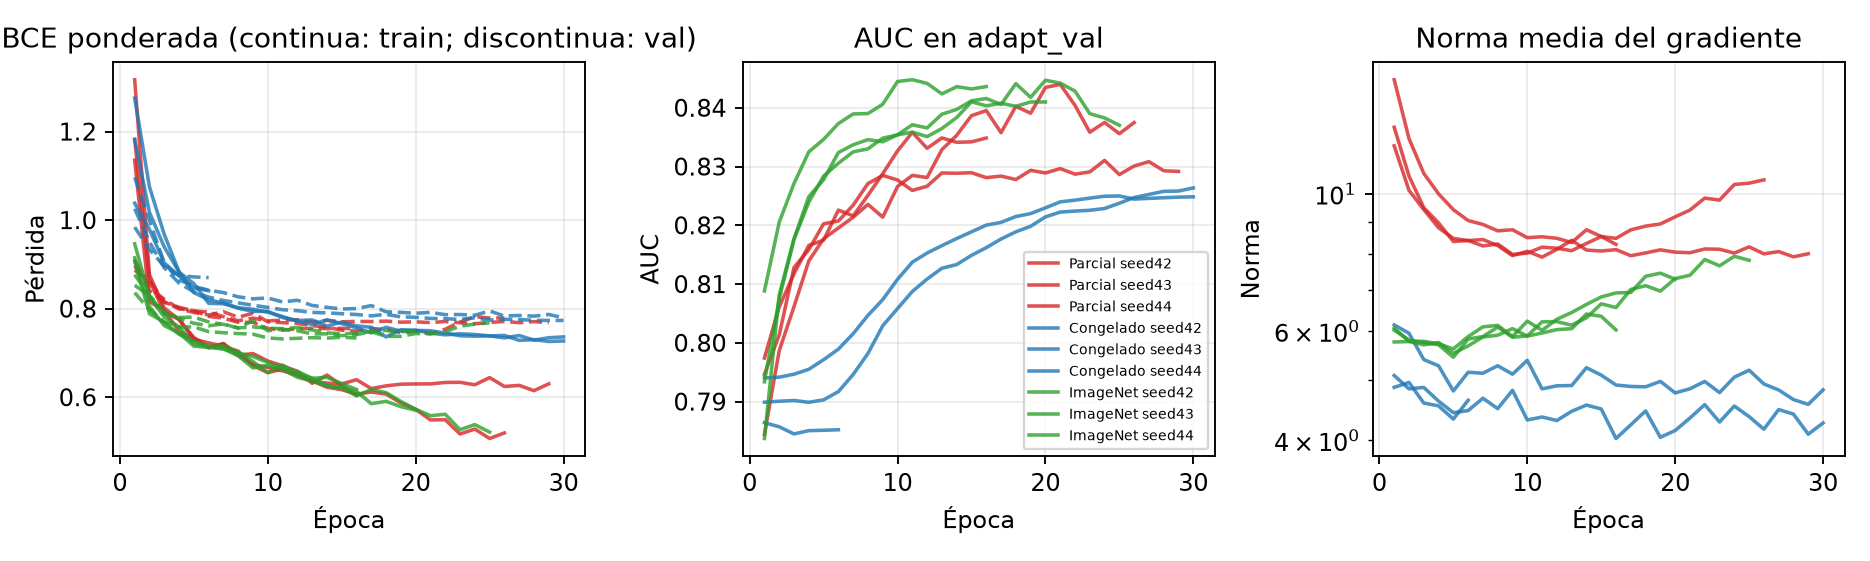
\includegraphics[width=\textwidth]{figures/nih_training_curves.png}
\caption{Dinámica del ajuste en NIH. Izquierda: pérdida de entrenamiento (continua) y de validación (discontinua). Centro: AUC en \texttt{adapt\_val}, criterio de parada. Derecha: norma media del gradiente.}\label{fig:curvas}
\end{figure}

La figura~\ref{fig:curvas} permite diagnosticar el sobreajuste con la curva clásica. En los modos parciales la pérdida de entrenamiento baja a 0,51--0,62, mientras la de validación se estanca en 0,73--0,78 desde la época 10: hay sobreajuste incipiente. La parada temprana sobre el AUC de validación lo contiene, porque retiene las épocas 11 a 24. En el congelado ambas pérdidas permanecen juntas: no sobreajusta, pero aprende despacio. Dos semillas llegan al tope de 30 épocas con la mejor época en la 25 y la 30, y la tercera se detuvo en la época 6, porque su AUC no superó el de la primera época en las cinco siguientes; eso explica su AUC de 0,832. La norma del gradiente se mantiene entre 4 y 15, sin picos ni colapso a cero; su aumento tardío en una corrida parcial coincide con el sobreajuste. La curva de datos escasos (figura~\ref{fig:curva}) muestra que con el 10\% de los pacientes ($\approx320$ imágenes) la CNN ya alcanza AUC $0{,}838\pm0{,}008$, por encima del Random Forest entrenado con todo (0,804), y que la ganancia no se ha saturado al 100\%.

\begin{figure}[h]\centering
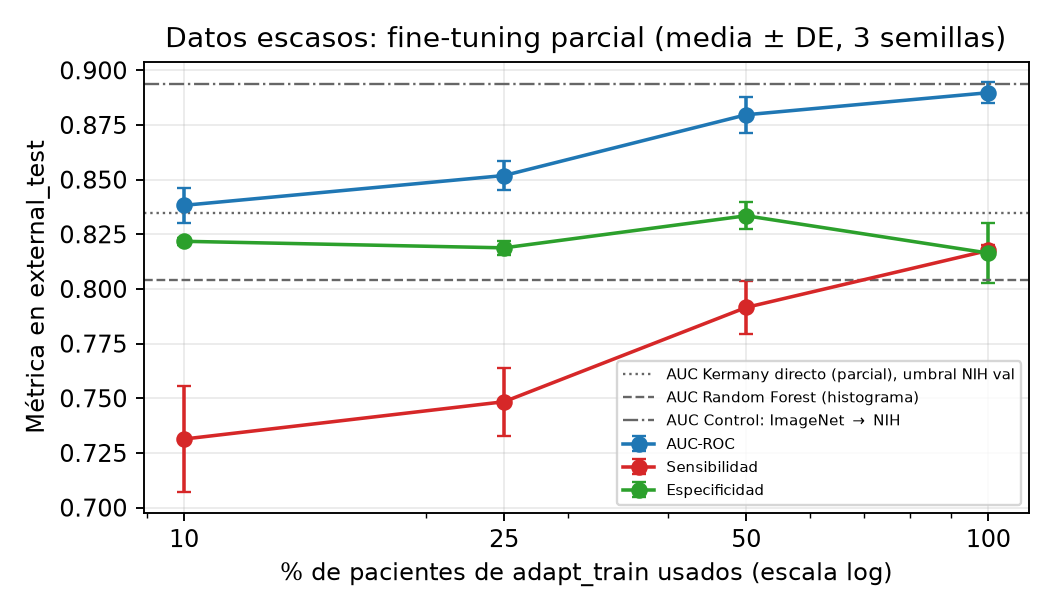
\includegraphics[width=.72\textwidth]{figures/learning_curve.png}
\caption{Desempeño en \texttt{external\_test} según la fracción de pacientes de \texttt{adapt\_train} usada (fine-tuning parcial desde Kermany). Las líneas horizontales son referencias de AUC.}\label{fig:curva}
\end{figure}

\textbf{Modelo final.} La regla, fijada antes de ver el test, es el máximo AUC medio en \texttt{adapt\_val}. La elige el fine-tuning parcial desde ImageNet: 0,843, frente a 0,837 del parcial desde Kermany y 0,813 del congelado. Es también la configuración más estable ($\pm0{,}002$) y cuesta lo mismo de entrenar (tabla~\ref{tab:costo}). La tabla~\ref{tab:config} resume su configuración. Se descongela solo el último bloque denso porque la distancia de dominio es grande: los bloques tempranos codifican bordes y texturas genéricos, útiles también en radiografías, mientras \texttt{denseblock4} combina rasgos de alto nivel propios de ImageNet que deben reaprenderse. Su tasa diez veces menor que la de la cabeza evita destruir esos pesos en las primeras épocas. Se audita la semilla 42: en test obtiene AUC 0,893, sensibilidad 0,846 y especificidad 0,806 con umbral 0,485, es decir, 314 verdaderos positivos, 57 falsos negativos, 216 falsos positivos y 897 verdaderos negativos. Frente al artículo se conservó el flujo y la ventaja de transferir desde ImageNet. Cambió el nivel de desempeño (AUC 0,89 frente a 0,99), y la tarea en adultos explica buena parte de ello: el 83\% de las neumonías de NIH coexisten con otros hallazgos, las etiquetas provienen de NLP y se mezclan vistas PA y AP.

\begin{table}[h]\centering\small
\caption{Configuración definitiva del modelo final (ImageNet $\rightarrow$ NIH, fine-tuning parcial).}\label{tab:config}
\begin{tabular}{ll}\toprule
Elemento & Decisión \\\midrule
Arquitectura y pesos & DenseNet121, ImageNet; cabeza lineal de una salida \\
Capas entrenables & \texttt{denseblock4}, \texttt{norm5} y cabeza (2.161.153 de 6.954.881 parámetros); BatchNorm congeladas en evaluación \\
Entrada & $224\times224$, gris replicado a RGB, normalización ImageNet \\
Aumento (solo entrenamiento) & Afín: $\pm10^\circ$, traslación y escala de 5\%; sin volteo \\
Pérdida & BCE ponderada, \texttt{pos\_weight} $=3$ (negativos/positivos de \texttt{adapt\_train}) \\
Optimizador & Adam, $10^{-4}$ en la cabeza y $10^{-5}$ en el bloque; \emph{weight decay} $10^{-4}$; lote de 16 \\
Parada & Máximo AUC en \texttt{adapt\_val}; ReduceLROnPlateau (factor 0,1, paciencia 2); paciencia 5; tope de 30 épocas \\
Umbral & Máxima sensibilidad con especificidad $\geq0{,}80$ en \texttt{adapt\_val} \\
Semillas & 42, 43 y 44; se audita la 42 \\\bottomrule
\end{tabular}
\end{table}

\section{Auditoría mediante explicabilidad}\label{sec:auditoria}
Se calcularon mapas Grad-CAM \parencite{selvaraju2017} sobre la última capa convolucional (tras \texttt{norm5}) y se midieron contra las 114 cajas del radiólogo. La energía del mapa dentro de la caja es el 9,2\% del total, para una caja que ocupa en promedio el 6,0\% de la imagen: una concentración de 1,40 veces lo esperado al azar. El máximo del mapa cae dentro de la caja en el 22\% de las imágenes, frente a un 9,8\% esperado al azar. La localización es real pero débil, e idéntica a la del modelo Kermany sin adaptar (1,40 y 22\%): el ajuste no la mejoró. En cambio, el modelo final pone el 50,5\% de su energía en el marco periférico (una franja del 10\% del lado en cada borde, el 35\% del área). El modelo Kermany pone ahí el 30,9\%. Esa es la zona de los marcadores de lateralidad y del texto \texttt{PORTABLE} que el hospital imprime en las placas AP (figura~\ref{fig:gradcam}, primera fila).

\begin{figure}[p]\centering
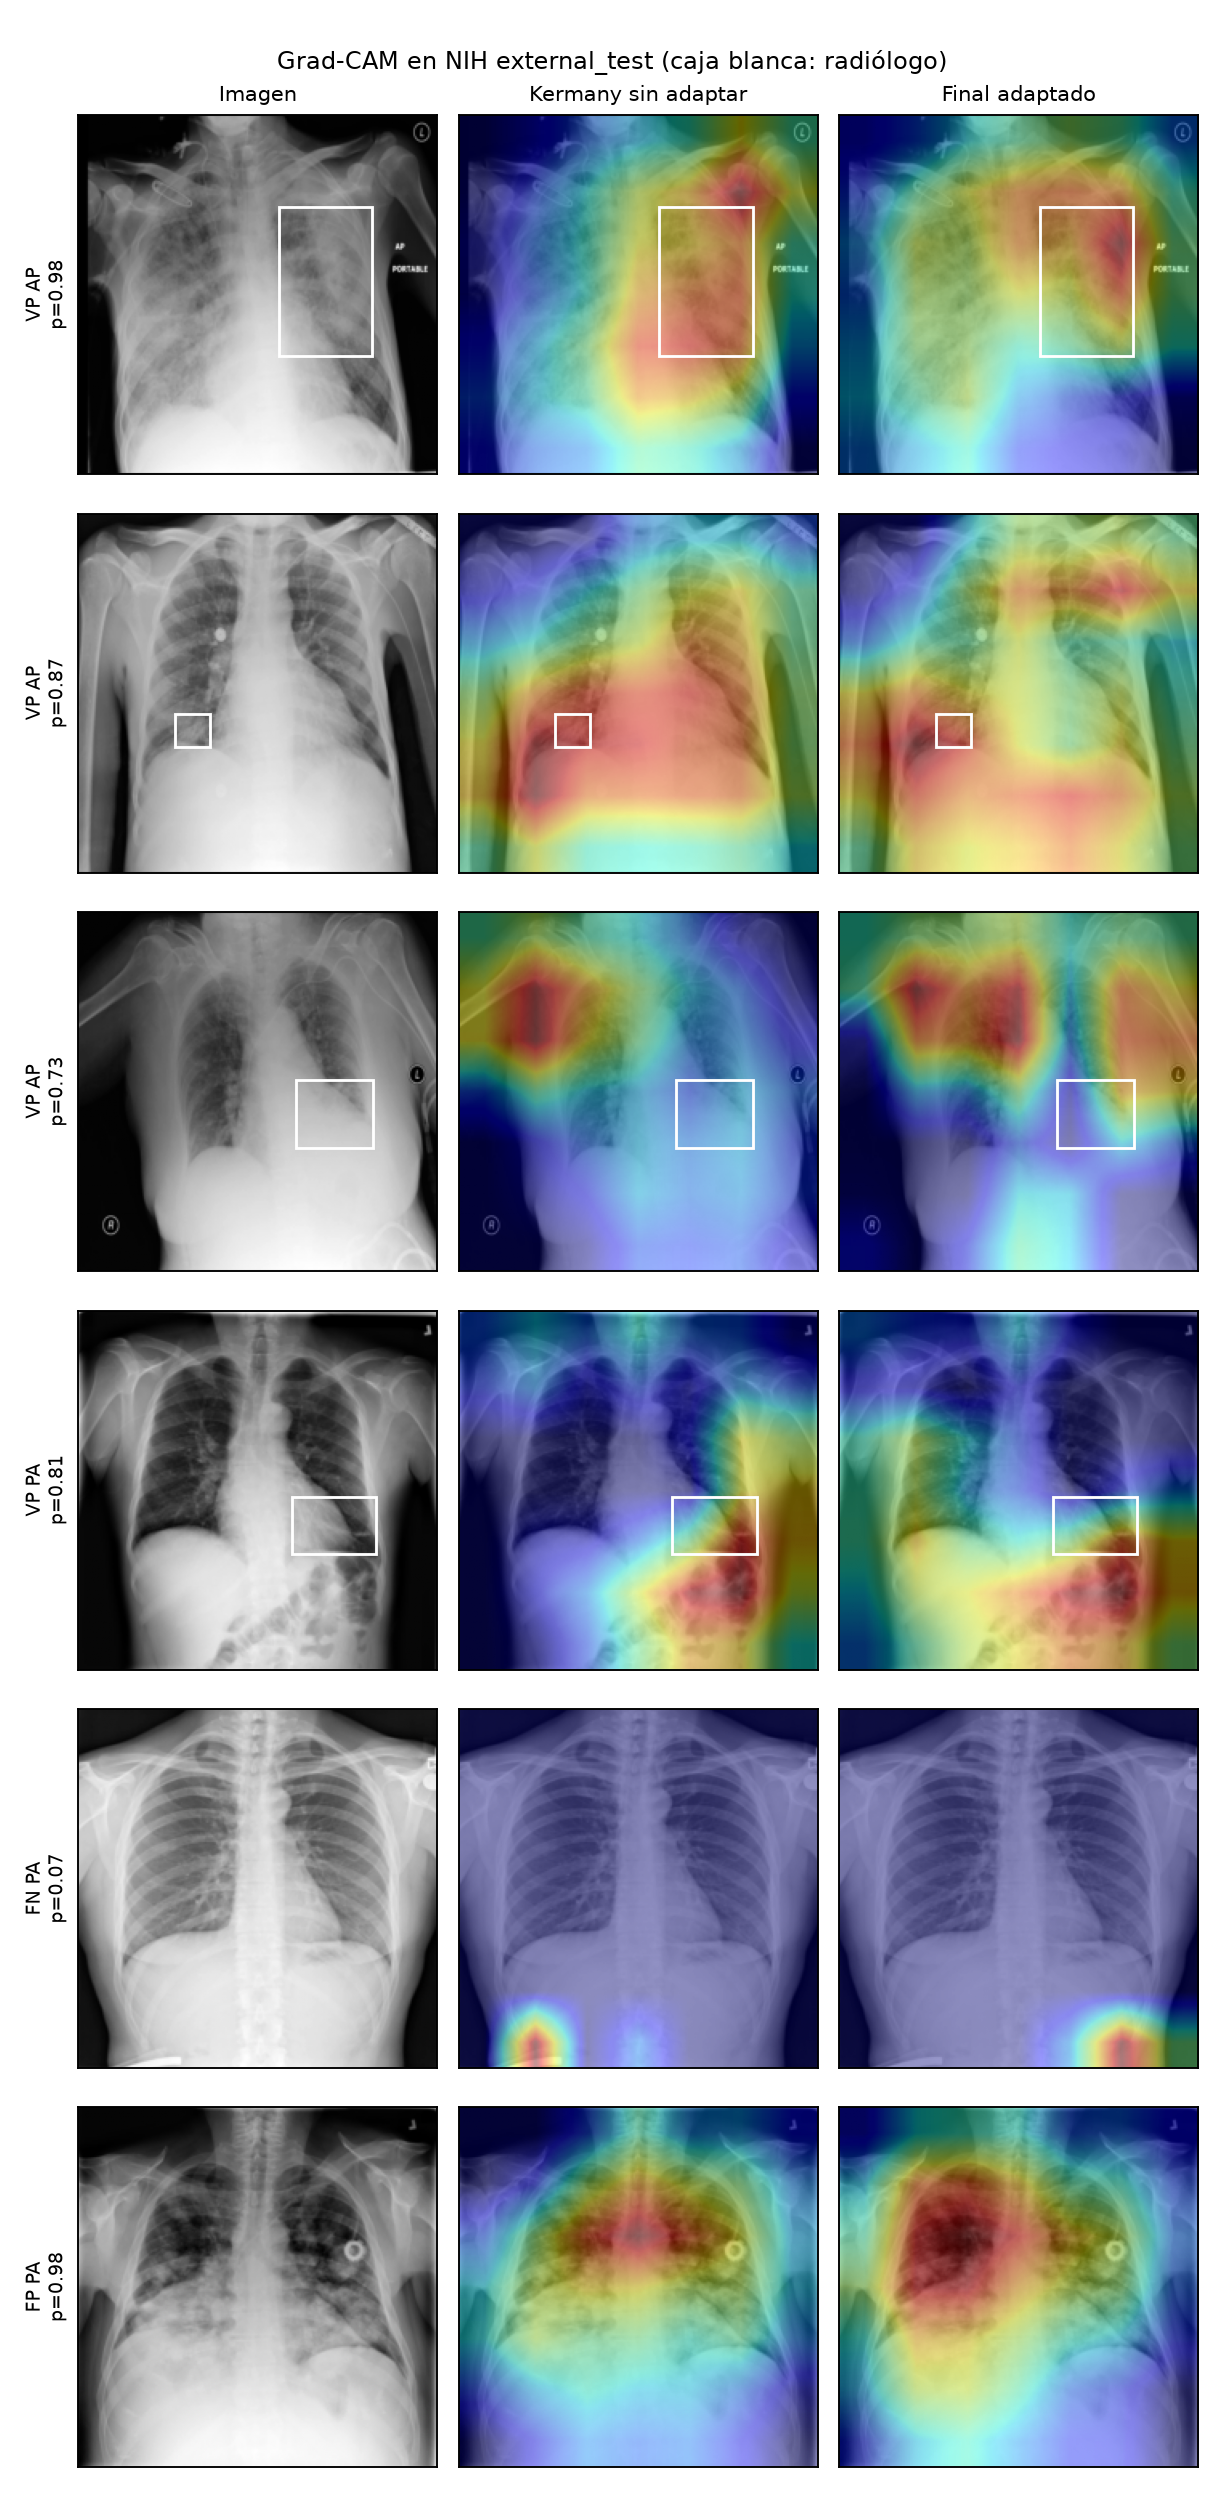
\includegraphics[height=.86\textheight]{figures/gradcam_examples.png}
\caption{Grad-CAM en \texttt{external\_test} para el modelo Kermany sin adaptar y el final. Caja blanca: radiólogo. VP, FN y FP indican verdadero positivo, falso negativo y falso positivo.}\label{fig:gradcam}
\end{figure}

Como un mapa no prueba causalidad, se diseñaron pruebas de respuesta conocida (tabla~\ref{tab:pruebas}). Ocluir la caja del radiólogo baja el puntaje una mediana de 0,075, frente a 0,011 al ocluir la región simétrica del otro pulmón. La caída es mayor en el 80\% de las imágenes (Wilcoxon $p<10^{-10}$): el modelo sí usa la lesión. Ocluir el 60\% central del tórax baja el AUC a 0,720 y no a 0,5. Fuera de los pulmones queda señal suficiente para ordenar casos, y ocluir solo ese mismo marco periférico desplaza la especificidad de 0,81 a 0,70. El volteo horizontal no altera el AUC (0,890).

\begin{table}[h]\centering\small
\caption{Pruebas de respuesta conocida y entradas fuera de dominio sobre el modelo final. ``Tasa de positivos'': fracción clasificada como neumonía con el umbral oficial.}\label{tab:pruebas}
\begin{tabular}{lccl}
\toprule
Prueba & AUC-ROC & Tasa de positivos & Respuesta esperada \\
\midrule
Original & 0{,}893 & 0{,}357 & Referencia \\
Tórax central ocluido (60\%) & 0{,}720 & 0{,}648 & AUC $\to$ 0,5 \\
Marco periférico ocluido (10\%) & 0{,}883 & 0{,}447 & AUC $\approx$ original \\
Volteo horizontal & 0{,}890 & 0{,}392 & AUC $\approx$ original \\
Kermany pediátrico (test) & 0{,}577 & 0{,}909 & Población no vista \\
\midrule
Gris uniforme (fuera de dominio) & -- & 1{,}000 & Sin positivos confiados \\
Ruido gaussiano (fuera de dominio) & -- & 1{,}000 & Sin positivos confiados \\
Radiografía invertida (fuera de dominio) & -- & 0{,}305 & Sin positivos confiados \\
Radiografía rotada $90^\circ$ (fuera de dominio) & -- & 0{,}915 & Sin positivos confiados \\
\bottomrule
\end{tabular}

\end{table}

El atajo más fuerte es la vista. En test, el 61\% de las neumonías son AP (placa portátil, paciente hospitalizado), frente al 19\% de los controles, de modo que la vista sola ya predice con AUC 0,71. Dentro de cada vista el modelo sigue discriminando (AUC 0,868 en AP y 0,844 en PA), así que no se reduce al atajo. Pero el punto de operación sí queda dominado por él. En AP la especificidad cae a 0,43; en PA la sensibilidad es 0,62 (tabla~\ref{tab:subgrupos}). \textbf{Dictamen de la auditoría:} el modelo aprendió señal pertinente, como prueban la oclusión de la lesión y la discriminación dentro de cada vista. Esa señal está mezclada con marcas de adquisición, la vista AP y los rótulos periféricos, que operan como atajo \parencite{zech2018,degrave2021} y que la cifra global oculta.

\section{Análisis de fallas, calibración y entradas fuera de dominio}\label{sec:fallas}
Los errores no se distribuyen al azar. De los 57 falsos negativos, el 96\% son PA, y el 32\% son neumonías sin otro hallazgo, el doble de su peso entre los positivos (17\%). La sensibilidad es 0,72 para la neumonía aislada y 0,87 cuando coexiste con otros hallazgos. El modelo se apoya en hallazgos acompañantes, una estratificación oculta propia de las etiquetas de NIH \parencite{oakdenrayner2020}. La neumonía con atelectasia se pierde en el 29\% de los casos, posiblemente porque ambas producen opacidades parecidas. De los 216 falsos positivos, el 56\% son AP, y la especificidad baja a 0,72 en mayores de 60 años. La falla es, a la vez, del modelo (atajo de vista), de los datos (etiquetas por NLP, vistas desbalanceadas por diseño caso-control) y del planteamiento (un único umbral para dos poblaciones de adquisición). En la práctica clínica, la mayoría de las alarmas en salas con placa portátil serían falsas y la neumonía leve en consulta ambulatoria (PA) se subdetectaría.

\begin{table}[h]\centering\small
\caption{Desempeño por subgrupo del modelo final en \texttt{external\_test}, con IC 95\% bootstrap por paciente.}\label{tab:subgrupos}
\begin{tabular}{lrrcc}
\toprule
Subgrupo & Imágenes & Positivas & Sensibilidad [IC 95\%] & Especificidad [IC 95\%] \\
\midrule
Todos & 1484 & 371 & 0{,}85 [0{,}80; 0{,}89] & 0{,}81 [0{,}78; 0{,}83] \\
Vista AP & 437 & 226 & 0{,}99 [0{,}98; 1{,}00] & 0{,}43 [0{,}36; 0{,}50] \\
Vista PA & 1047 & 145 & 0{,}62 [0{,}53; 0{,}71] & 0{,}89 [0{,}87; 0{,}91] \\
Mujer & 640 & 129 & 0{,}82 [0{,}74; 0{,}89] & 0{,}82 [0{,}78; 0{,}85] \\
Hombre & 844 & 242 & 0{,}86 [0{,}80; 0{,}91] & 0{,}80 [0{,}76; 0{,}83] \\
Edad 18-39 & 518 & 136 & 0{,}83 [0{,}74; 0{,}90] & 0{,}87 [0{,}83; 0{,}90] \\
Edad 40-59 & 662 & 163 & 0{,}86 [0{,}79; 0{,}92] & 0{,}80 [0{,}76; 0{,}83] \\
Edad >=60 & 304 & 72 & 0{,}85 [0{,}76; 0{,}93] & 0{,}72 [0{,}67; 0{,}78] \\
Neumonía sola & 64 & 64 & 0{,}72 & -- \\
Neumonía + co-hallazgos & 307 & 307 & 0{,}87 & -- \\
\bottomrule
\end{tabular}

\end{table}

\begin{figure}[h]\centering
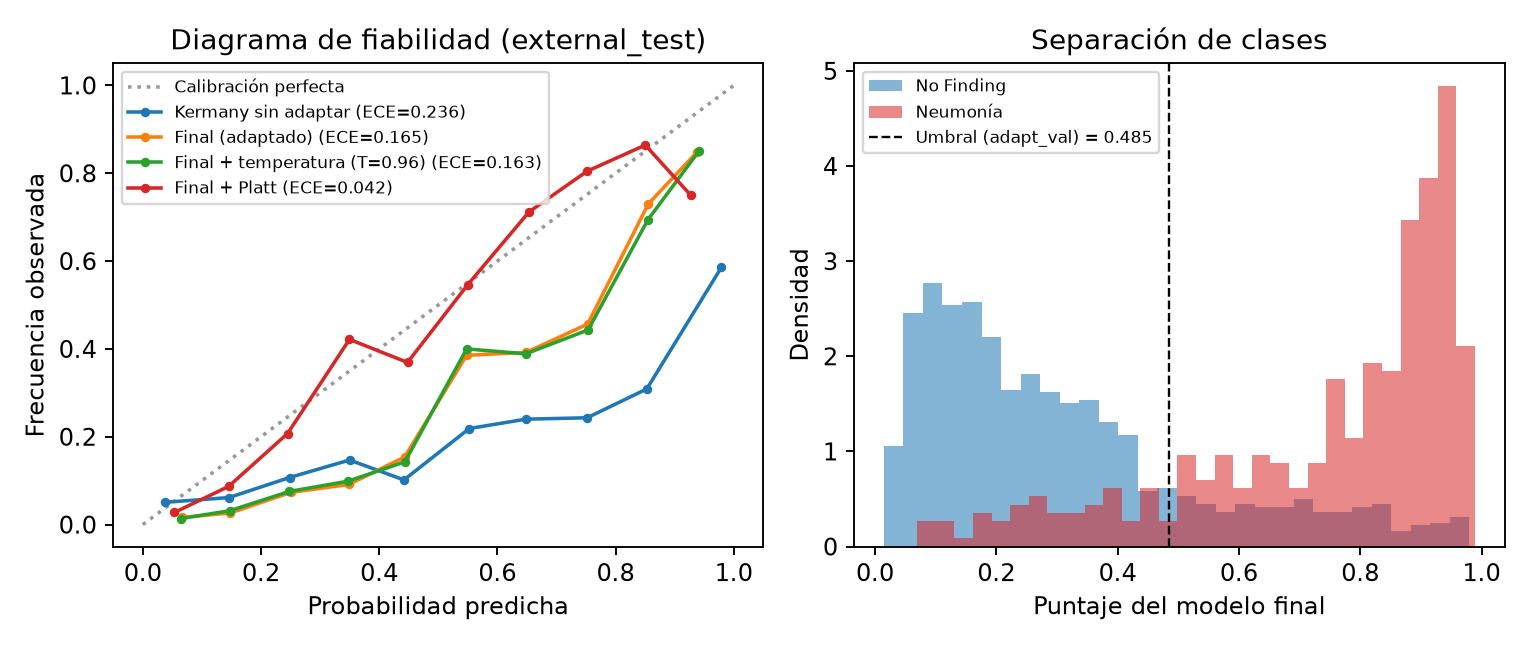
\includegraphics[width=.92\textwidth]{figures/calibration.png}
\caption{Izquierda: diagrama de fiabilidad; la temperatura y Platt se ajustan solo en \texttt{adapt\_val}. Derecha: distribución del puntaje del modelo final por clase y umbral oficial.}\label{fig:calibracion}
\end{figure}

\textbf{Calibración.} El modelo final sobreestima la probabilidad en todo el rango (figura~\ref{fig:calibracion}). Predice en promedio 0,415 para una prevalencia de 0,25, con ECE 0,165 y Brier 0,139. La causa es la BCE ponderada con \texttt{pos\_weight} $=3$, que desplaza los logits en $\log 3$. El escalado por temperatura \parencite{guo2017} no corrige un desplazamiento: con $T=0{,}96$ el ECE apenas cambia (0,163). El escalado de Platt \parencite{platt1999}, ajustado en \texttt{adapt\_val}, sí lo corrige. Su intercepto ($-1{,}02$) coincide con $-\log 3$, y el ECE baja a 0,042 y el Brier a 0,108, sin alterar las decisiones, porque la transformación es monótona. Con sensibilidad y especificidad fijas, el valor predictivo positivo es 0,59 a la prevalencia del diseño, 0,33 al 10\% y 0,08 al 2\%; el negativo es $\geq0{,}94$ en todos los casos. El modelo sirve más para descartar que para confirmar.

\textbf{Fuera de dominio.} El modelo no tiene mecanismo de rechazo. Una imagen gris uniforme, ruido gaussiano y radiografías rotadas $90^\circ$ se clasifican como neumonía en el 100\%, 100\% y 92\% de los casos, con puntajes medianos de 0,63 a 0,74. Sobre el test pediátrico de Kermany, población que el modelo final nunca vio, el AUC es 0,577: lo aprendido en adultos no se devuelve a niños.

\section{Dictamen sobre la profundidad}
\textbf{La arquitectura profunda sí se justifica para este problema, con tres condiciones.} A favor:
\begin{itemize}
\item \emph{Comparación.} En NIH el modelo final supera al Random Forest por 0,09 de AUC y 20--22 puntos de sensibilidad a especificidad comparable, en las tres semillas y con intervalos pareados que excluyen el cero; en Kermany la ventaja se repite: $+6$ puntos de sensibilidad y $+0{,}05$ de AUC.
\item \emph{Datos.} Con solo el 10\% de los pacientes locales ya supera a la línea base entrenada con el 100\%; la transferencia hace rendir pocos datos.
\item \emph{Costo} (tabla~\ref{tab:costo}). Ajustar en NIH cuesta 10--12 minutos por corrida en una GPU de 4 GB. Descongelar \texttt{denseblock4} multiplica por 2.100 los parámetros entrenables, pero apenas alarga la época (30 frente a 28 s en NIH; 39 s en ambos modos en Kermany), porque el cuello de botella es la carga de datos. En Kermany, al converger antes, incluso entrena menos minutos (15,3 frente a 19,9). La inferencia es la misma red en ambos modos: las medianas (19,5--21,1 ms) tienen IQR solapados, de modo que la diferencia de la Fase 2 (13,7 frente a 11,9 ms) no reflejaba un costo distinto.
\end{itemize}
Las condiciones vienen de la auditoría:
\begin{enumerate}
\item basta transferir desde ImageNet; el paso por Kermany no se justifica;
\item el modelo sirve para ordenar casos, no para un diagnóstico autónomo, porque mezcla señal clínica con el atajo de la vista;
\item requiere calibración de Platt y umbrales evaluados por vista antes de cualquier uso.
\end{enumerate}

\begin{table}[h]\centering\small
\caption{Costo de entrenamiento e inferencia (medias de tres semillas, GPU GTX 1650). La latencia es la mediana de 100 inferencias de una imagen, con IQR.}\label{tab:costo}
\begin{tabular}{llrrrc}
\toprule
Etapa & Configuración & Parám. entrenables & Épocas & Min. entren. & Latencia ms [IQR] \\
\midrule
Kermany & Congelado & 1.025 & 30{,}0 & 19{,}9 & 20{,}7 [20{,}0; 23{,}5] \\
Kermany & Fine-tuning parcial & 2.161.153 & 21{,}3 & 15{,}3 & 21{,}1 [20{,}4; 25{,}2] \\
NIH & Fine-tuning parcial & 2.161.153 & 23{,}7 & 12{,}0 & 19{,}5 [18{,}8; 22{,}7] \\
NIH & Congelado & 1.025 & 22{,}0 & 10{,}2 & 20{,}1 [19{,}2; 23{,}7] \\
NIH & ImageNet, parcial & 2.161.153 & 20{,}3 & 10{,}5 & 19{,}8 [19{,}1; 22{,}3] \\
\bottomrule
\end{tabular}

\end{table}

\section{Limitaciones y proyección}\label{sec:limites}
\textbf{Limitaciones.}
\begin{itemize}
\item \emph{Representatividad.} NIH es un único hospital estadounidense: no hay evidencia sobre población colombiana, y el diseño caso-control con prevalencia de 0,25 no reproduce la de ningún servicio.
\item \emph{Etiquetas.} Provienen de NLP sobre informes, sin confirmación clínica.
\item \emph{Validación.} Hay una sola partición externa y tres semillas por configuración. La auditoría de Grad-CAM cubre solo 114 imágenes con caja, y la resolución $7\times7$ del mapa limita la localización fina.
\item \emph{Arquitectura y herramientas.} Por cómputo se redujo DenseNet201 a DenseNet121, y se usó PyTorch en lugar de TensorFlow/Keras (sección~\ref{sec:declaracion}).
\item \emph{Umbrales por vista.} Se probaron como análisis exploratorio y no se adoptaron, para no cambiar el protocolo después de ver el test. Elegidos en \texttt{adapt\_val}, equilibran las vistas: sensibilidad 0,80 y especificidad 0,76 en AP, 0,72 y 0,83 en PA. A cambio, la sensibilidad global baja de 0,85 a 0,77.
\end{itemize}

\textbf{Continuidad.} El protocolo está listo para BRAX o datos colombianos: basta reemplazar el manifiesto. Otras líneas son el entrenamiento estratificado por vista y una formulación multietiqueta que separe la neumonía de sus co-hallazgos.

\textbf{MLOps.} Llevar el modelo a producción exigiría:
\begin{itemize}
\item \emph{Versionamiento} conjunto de datos (manifiestos con SHA-256 y CRC32, ya implementado), código (git) y modelos (\emph{checkpoint} con su \texttt{run\_config.json} en un registro de modelos).
\item Una \emph{compuerta de entrada} que rechace imágenes fuera de dominio, con verificación DICOM de vista y modalidad y un detector OOD, ya que hoy el modelo no rechaza nada.
\item \emph{Monitoreo} de la proporción AP/PA, de las estadísticas de intensidad y de la distribución del puntaje, con alertas de deriva (por ejemplo, PSI) y revisión humana de una muestra.
\item \emph{Recalibración} con la prevalencia local antes del despliegue y cada vez que se detecte deriva.
\end{itemize}
Las ejecuciones largas ya corren bajo un supervisor que reinicia etapas atascadas (\texttt{make resume}), un primer paso hacia esa orquestación.

\section{Declaración de herramientas y uso de inteligencia artificial}\label{sec:declaracion}
\begin{itemize}
\item \emph{Marco de trabajo.} Se usó PyTorch 2.7 en lugar de TensorFlow/Keras, por continuidad con la Fase 2; los historiales CSV y sus figuras cumplen la función de TensorBoard.
\item \emph{Datos.} Las etiquetas de NIH provienen de su repositorio oficial; las imágenes, del espejo público \texttt{alkzar90/NIH-Chest-X-ray-dataset} de Hugging Face, porque los enlaces originales ya no responden. Cada imagen se verificó por CRC32.
\item \emph{Inteligencia artificial generativa.} Se empleó Claude (Anthropic), mediante Claude Code, como apoyo para escribir y depurar código, diagnosticar errores y redactar borradores. El equipo revisó cada resultado, y todas las cifras provienen de los artefactos versionados en el repositorio.
\end{itemize}

\printbibliography

\appendix
\section{Respuesta a la retroalimentación de la Fase 2}\label{anx:matriz}
\begin{table}[h]\centering\small
\begin{tabular}{>{\raggedright}p{6.2cm}>{\raggedright\arraybackslash}p{10.3cm}}\toprule
Observación & Respuesta en esta entrega \\\midrule
El traslado al conjunto local no se ejecutó & Traslado real a NIH: nueve corridas de ajuste, evaluación directa y curva de datos escasos (sección 3.2). \\
No hay evidencia de generalización a adultos brasileños & Sin acceso a BRAX no puede evaluarse: NIH mide el paso niños $\rightarrow$ adultos y China $\rightarrow$ EE.\,UU., no la población latinoamericana. Se declara como limitación (sección~\ref{sec:limites}) y el protocolo queda listo para BRAX. \\
La estrategia local quedó como plan & Congelado frente a parcial en NIH con bootstrap pareado, más control desde ImageNet (sección 3.2, anexo~\ref{anx:pareado}). \\
Explicar la caída de especificidad 0,970 $\rightarrow$ 0,869 & Se prueban el punto de operación y la partición por imagen (sección 3.1, tabla~\ref{tab:replica}); tras corregir la fuga, la cifra es 0,852. \\
Falta pérdida de validación & Se registra en todas las corridas y se usa para diagnosticar el sobreajuste: Kermany en la sección 3.1, NIH en la figura~\ref{fig:curvas}. \\
Variabilidad entre semillas como estabilidad & Se interpreta como estabilidad del entrenamiento (sección 3.2). \\
Especificidad puntual $<0{,}80$ no cumple & La corrida congelada con semilla 42 en Kermany (0,797) se declara como incumplimiento (sección 3.1). \\
Separar costo de entrenamiento e inferencia & Tabla~\ref{tab:costo} y sección 6. \\
No sobreinterpretar 13,7 frente a 11,9 ms & Latencia sincronizada con IQR; las diferencias no son reales (sección 6). \\\bottomrule
\end{tabular}
\end{table}

\section{Diferencias pareadas en NIH}\label{anx:pareado}
\begin{table}[h]\centering\small
\caption{Diferencias A $-$ B en puntos porcentuales (AUC en centésimas) con IC 95\% bootstrap pareado por paciente en \texttt{external\_test}.}
\begin{tabular}{llccc}
\toprule
Contraste (A $-$ B) & Semilla & $\Delta$ Sens. & $\Delta$ Espec. & $\Delta$ AUC \\
\midrule
Parcial $-$ RF & 42 & 17{,}5 [12{,}5; 23{,}4] & -1{,}3 [-3{,}9; 1{,}2] & 8{,}2 [5{,}6; 10{,}7] \\
Parcial $-$ RF & 43 & 18{,}1 [12{,}8; 23{,}5] & 1{,}5 [-0{,}8; 4{,}2] & 9{,}2 [6{,}5; 11{,}8] \\
Parcial $-$ RF & 44 & 18{,}1 [13{,}0; 23{,}7] & -1{,}3 [-3{,}9; 1{,}3] & 8{,}3 [5{,}7; 10{,}8] \\
Congelado $-$ RF & 42 & 17{,}5 [13{,}0; 22{,}2] & -0{,}9 [-3{,}4; 1{,}5] & 7{,}8 [5{,}3; 10{,}4] \\
Congelado $-$ RF & 43 & 17{,}5 [13{,}0; 22{,}0] & -1{,}0 [-3{,}4; 1{,}6] & 7{,}8 [5{,}2; 10{,}3] \\
Congelado $-$ RF & 44 & 6{,}2 [1{,}6; 10{,}7] & 0{,}4 [-2{,}2; 3{,}1] & 2{,}8 [0{,}0; 5{,}6] \\
Parcial $-$ congelado & 42 & 0{,}0 [-3{,}5; 3{,}8] & -0{,}4 [-2{,}1; 1{,}2] & 0{,}4 [-0{,}6; 1{,}3] \\
Parcial $-$ congelado & 43 & 0{,}5 [-2{,}6; 3{,}8] & 2{,}5 [0{,}5; 4{,}2] & 1{,}5 [0{,}5; 2{,}4] \\
Parcial $-$ congelado & 44 & 11{,}9 [7{,}6; 16{,}5] & -1{,}8 [-3{,}9; 0{,}5] & 5{,}5 [3{,}6; 7{,}3] \\
Kermany $\to$ NIH $-$ ImageNet $\to$ NIH & 42 & -3{,}2 [-6{,}1; -0{,}7] & 0{,}1 [-1{,}5; 1{,}7] & -0{,}6 [-1{,}4; 0{,}1] \\
Kermany $\to$ NIH $-$ ImageNet $\to$ NIH & 43 & -3{,}5 [-6{,}1; -1{,}1] & 2{,}7 [1{,}1; 4{,}3] & 0{,}0 [-0{,}7; 0{,}6] \\
Kermany $\to$ NIH $-$ ImageNet $\to$ NIH & 44 & -1{,}6 [-4{,}3; 0{,}8] & 0{,}3 [-1{,}5; 2{,}1] & -0{,}5 [-1{,}2; 0{,}2] \\
\bottomrule
\end{tabular}

\end{table}
\end{document}
